\documentclass[compress]{beamer}
\usepackage{ifthen,verbatim}

\newcommand{\isnote}{}
\xdefinecolor{lightyellow}{rgb}{1.,1.,0.25}
\xdefinecolor{darkblue}{rgb}{0.1,0.1,0.7}

%% Uncomment this to get annotations
%% \def\notes{\addtocounter{page}{-1}
%%            \renewcommand{\isnote}{*}
%% 	   \beamertemplateshadingbackground{lightyellow}{white}
%%            \begin{frame}
%%            \frametitle{Notes for the previous page (page \insertpagenumber)}
%%            \itemize}
%% \def\endnotes{\enditemize
%% 	      \end{frame}
%%               \beamertemplateshadingbackground{white}{white}
%%               \renewcommand{\isnote}{}}

%% Uncomment this to not get annotations
\def\notes{\comment}
\def\endnotes{\endcomment}

\setbeamertemplate{navigation symbols}{}
\setbeamertemplate{headline}{\mbox{ } \hfill
\begin{minipage}{5.5 cm}
\vspace{-0.75 cm} \small
\end{minipage} \hfill
\begin{minipage}{4.5 cm}
\vspace{-0.75 cm} \small
\begin{flushright}
\ifthenelse{\equal{\insertpagenumber}{1}}{}{Jim Pivarski \hspace{0.2 cm} \insertpagenumber\isnote/\pageref{numpages}}
\end{flushright}
\end{minipage}\mbox{\hspace{0.2 cm}}\includegraphics[height=1 cm]{../cmslogo} \hspace{0.1 cm} \includegraphics[height=1 cm]{../tamulogo} \hspace{0.01 cm} \vspace{-1.05 cm}}

\begin{document}
\begin{frame}
\vfill
\begin{center}
\textcolor{darkblue}{\Large Suppressing Fake Dimuons from ME1/1a Triplets}

\vfill
\begin{columns}
\column{0.3\linewidth}
\begin{center}
\large
Jim Pivarski
\end{center}
\end{columns}

\begin{columns}
\column{0.3\linewidth}
\begin{center}
\scriptsize
{\it Texas A\&M University}
\end{center}
\end{columns}

\vfill
 3 May, 2010

\end{center}
\end{frame}

%% \begin{notes}
%% \item This is the annotated version of my talk.
%% \item If you want the version that I am presenting, download the one
%% labeled ``slides'' on Indico (or just ignore these yellow pages).
%% \item The annotated version is provided for extra detail and a written
%% record of comments that I intend to make orally.
%% \item Yellow notes refer to the content on the {\it previous} page.
%% \item All other slides are identical for the two versions.
%% \end{notes}

\small

\begin{frame}
\frametitle{Motivation}

\begin{columns}
\column{0.7\linewidth}
\begin{itemize}
\item Groups of near-by muons are a typical signature of hidden valley
  models used to explain PAMELA positron excess

\item For details, see {\it Lepton Jets as a Signature for Dark Matter} {\scriptsize (C.\ Boulahouache, March 16 Exotica)}

\href{http://indico.cern.ch/materialDisplay.py?contribId=2&materialId=slides&confId=87421}{\scriptsize http://indico.cern.ch/materialDisplay.py?}

\vspace{-0.2 cm}
\href{http://indico.cern.ch/materialDisplay.py?contribId=2&materialId=slides&confId=87421}{\scriptsize contribId=2\&materialId=slides\&confId=87421}

\item Problem: we're already seeing fake ``muon jets'' due to ganging of ME1/1a strips:

\end{itemize}

\column{0.3\linewidth}
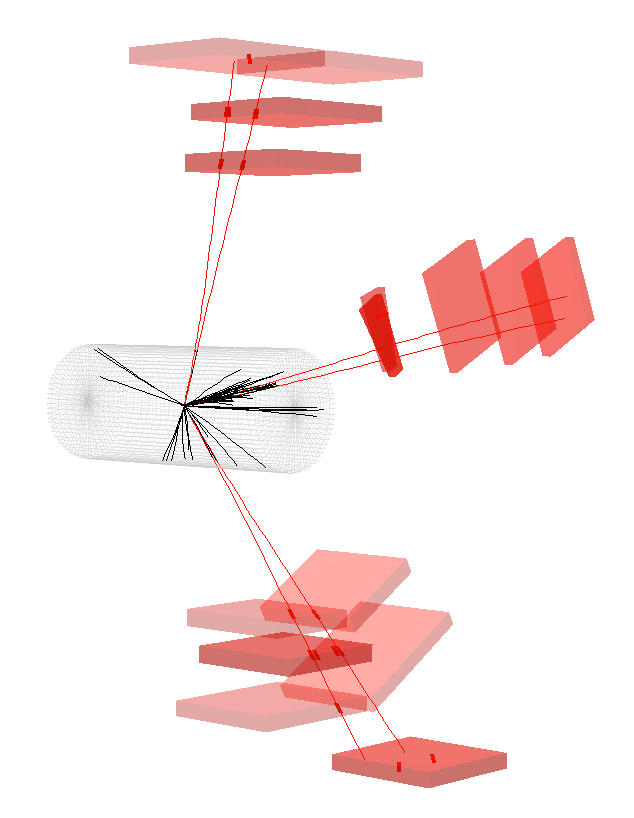
\includegraphics[width=\linewidth]{eventdisplay_3d.png}

\mbox{ } \hfill {\tiny event from a $U(1)_{\mbox{\tiny dark}}$ model} \hfill \mbox{ }
\end{columns}

\vfill
\begin{columns}
\column{0.6\linewidth}

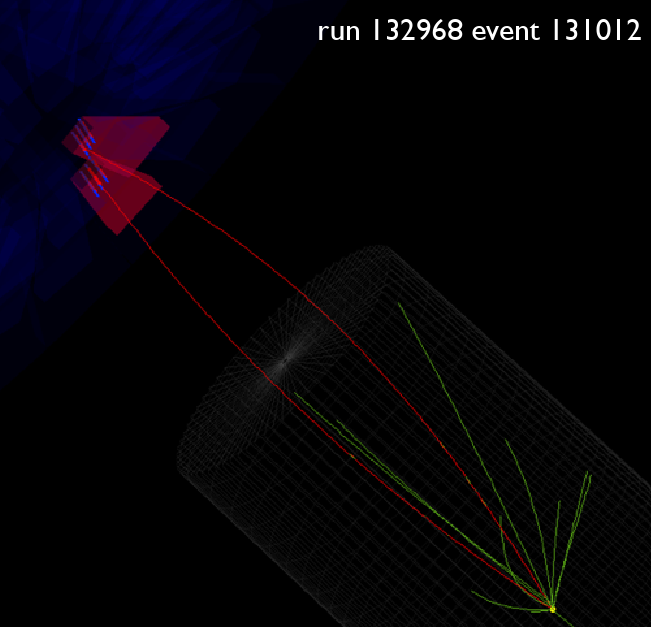
\includegraphics[height=3 cm]{triplet.png} \hfill 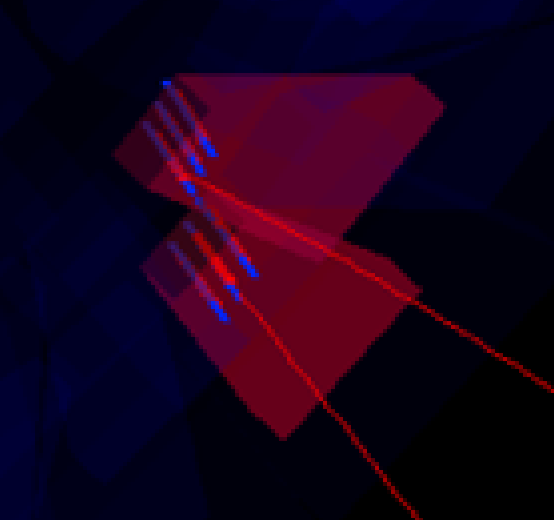
\includegraphics[height=3 cm]{triplet_closeup.png}

\hfill \scriptsize N.\ Kypreos

\column{0.4\linewidth}
\begin{itemize}
\item One real muon produces three parallel segments in each ME1/1a chamber

\item Non-muon tracks can be associated with the other segments
\end{itemize}
\end{columns}
\end{frame}

\begin{frame}
\frametitle{Scalpel-cut for ME1/1a triplets}

\begin{itemize}
\item D.\ Kovalskyi and N.\ Kypreos have shown ways to suppress
  backgrounds from muons that approach or overlap each other

\href{http://indico.cern.ch/conferenceDisplay.py?confId=88576}{\scriptsize http://indico.cern.ch/conferenceDisplay.py?confId=88576}

\item However, these methods might eliminate legitimate muon jets

\item The effect: strip number mod 16 are read out of the same channel, triplicating hits with an offset of $16 \times 3.88$~mrad

\item Differences in matched segment $\phi$ position for dimuons in ME1/1a:
\end{itemize}

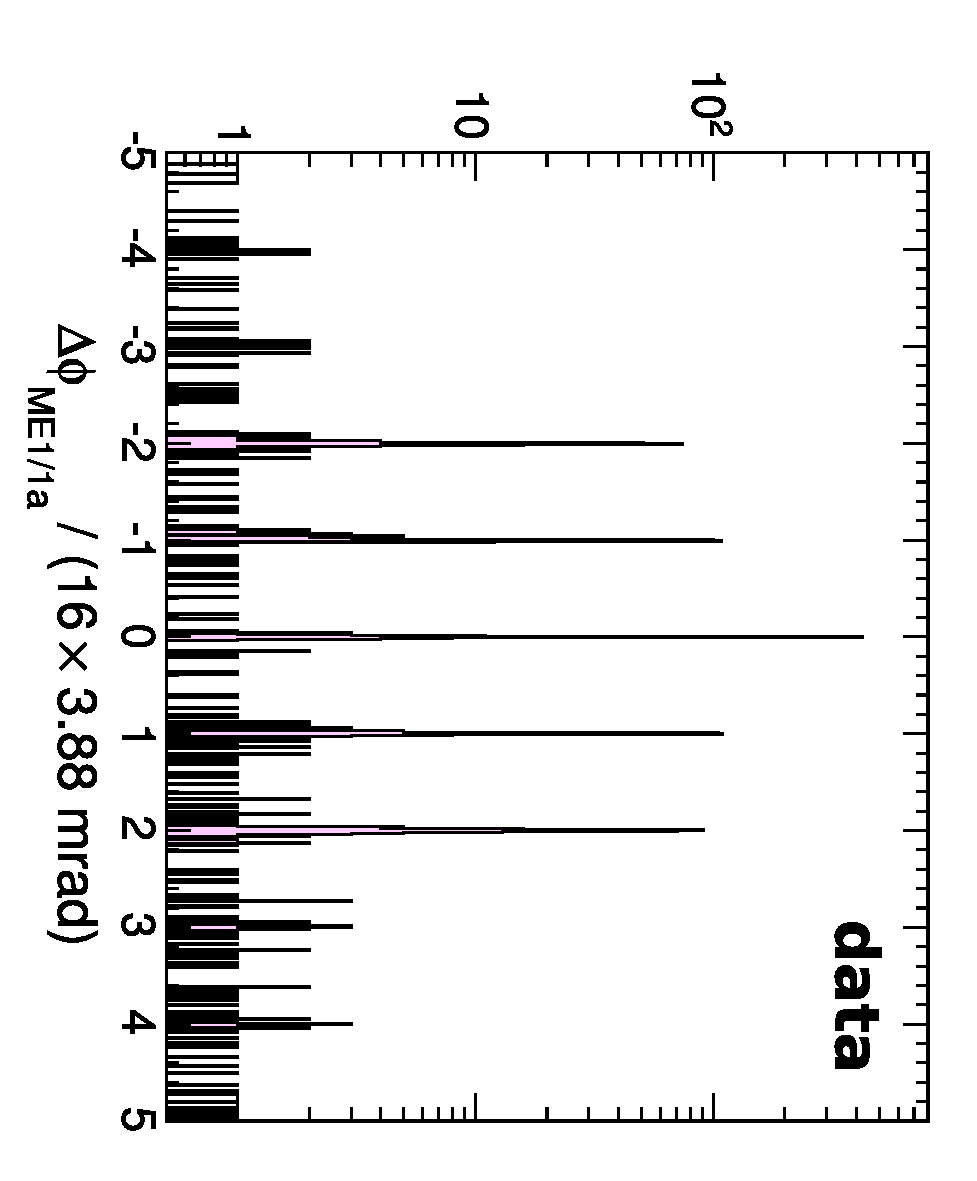
\includegraphics[height=0.5\linewidth, angle=90]{gangedstripcut.pdf} 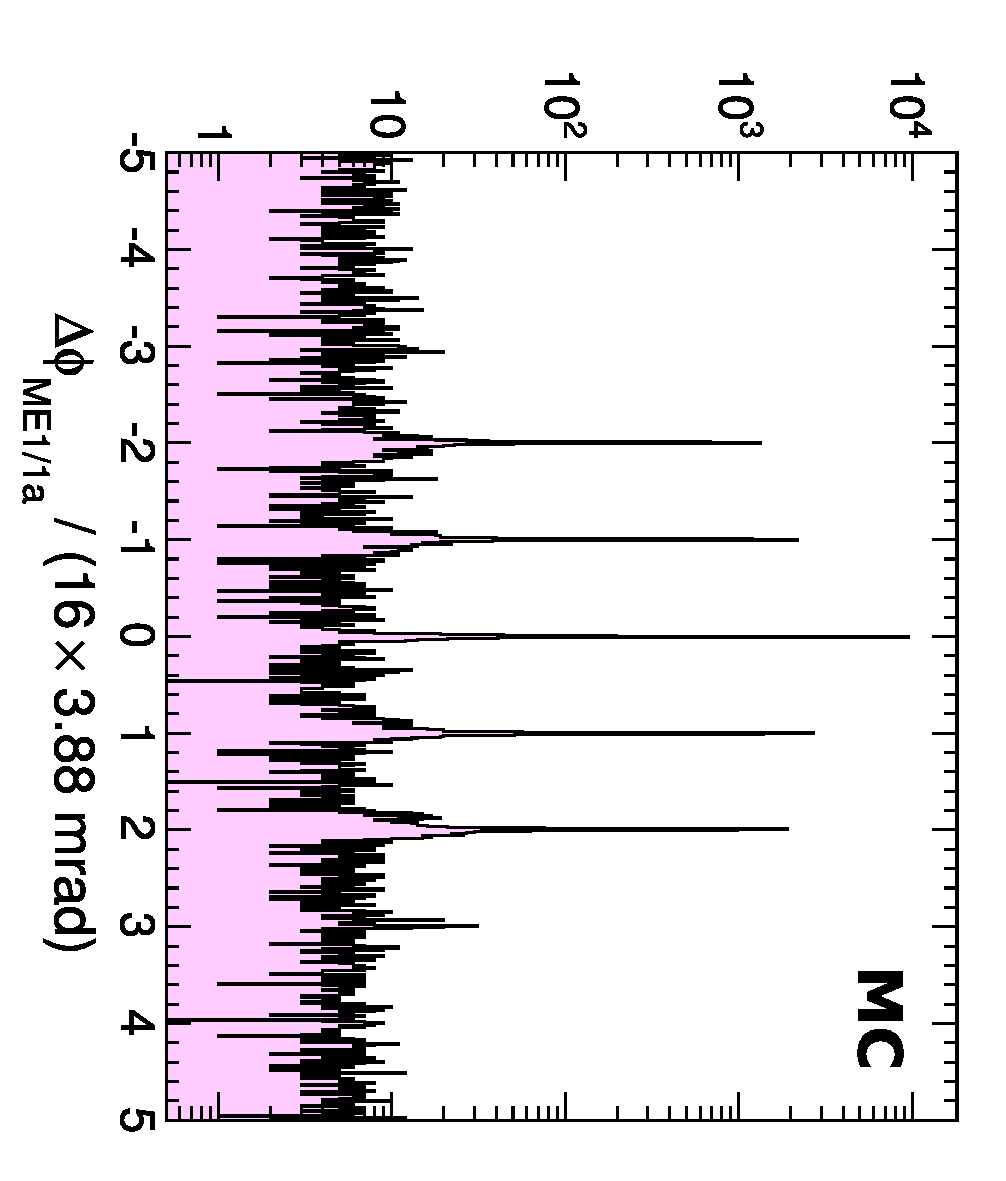
\includegraphics[height=0.5\linewidth, angle=90]{gangedstripcut_MC.pdf}
\end{frame}

\begin{frame}[fragile]
\frametitle{Implementing the cut}

{\bf Method 1:}

\begin{verbatim}
int stripnumber = cscGeometry->layer(layerId)->geometry()
  ->nearestStrip(LocalPoint(segMatch->x, segMatch->y, 0.));
long channel = chamberId.rawId()*16 + ((strip-1) % 16);
\end{verbatim}

\vspace{-0.2 cm}
and make sure the two muons don't share a ``channel''.

\vfill
{\bf Method 2:}
\begin{verbatim}
const Surface &s = cscGeometry->idToDet(chamberId)->surface();
GlobalPoint point =
  s.toGlobal(LocalPoint(segMatch->x, segMatch->y, 0.));
GlobalVector direction =
  s.toGlobal(LocalVector(segMatch->dXdZ, segMatch->dYdZ, 1.));
\end{verbatim}

\vspace{-0.2 cm}
linearly extrapolate to a common $z$-plane (e.g.\ 602.3 cm), and make
sure they don't overlap with a small tolerance (plots on previous page).

\vfill
Both methods require access to CSCGeometry.
\end{frame}

\begin{frame}
\frametitle{Results}

\begin{itemize}
\item trackerMuons only (from a Muon collection with only trackerMuons)

\item Quality cuts (following N.\ Kypreos and M.\ Chen):
\begin{itemize}\setlength{\itemsep}{0.1 cm}
\item \scriptsize  $p_T > 1$~GeV/$c$, $|\vec{p}| > 2.5$~GeV/$c$
\item \scriptsize $N_{\mbox{\scriptsize tracker hits}} > 12$, $\chi^2/N_{\mbox{\scriptsize dof}} < 5$
\item \scriptsize $|d_{xy}| < 0.5$~cm, $|d_{z}| < 5$~cm, 
\item \scriptsize TMLastStationAngTight
\item \scriptsize trigger bit 40 or 41, not beam-halo, physics declared, no beam scraping
\end{itemize}

\item Ganged strip sharing cut (method 1) significantly reduces background with little effect on $J/\psi$ and $\phi(1020)$
\end{itemize}

\begin{columns}
\column{0.65\linewidth}
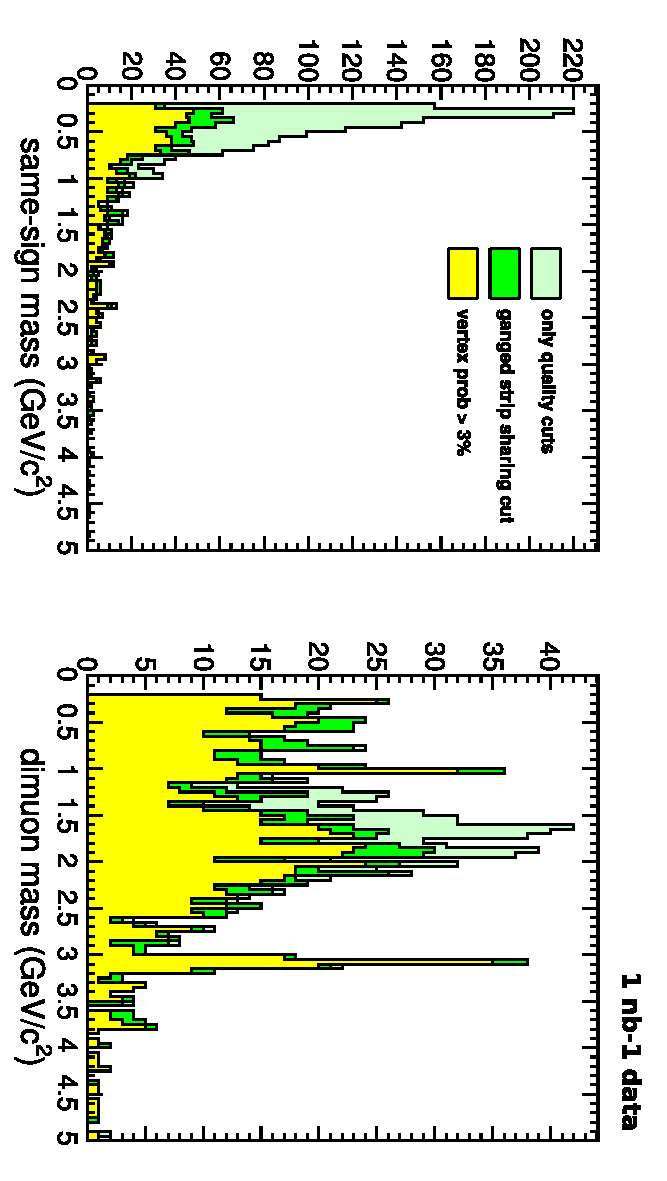
\includegraphics[height=\linewidth, angle=90]{gangedstripcut_mass.pdf}

\column{0.5\linewidth}
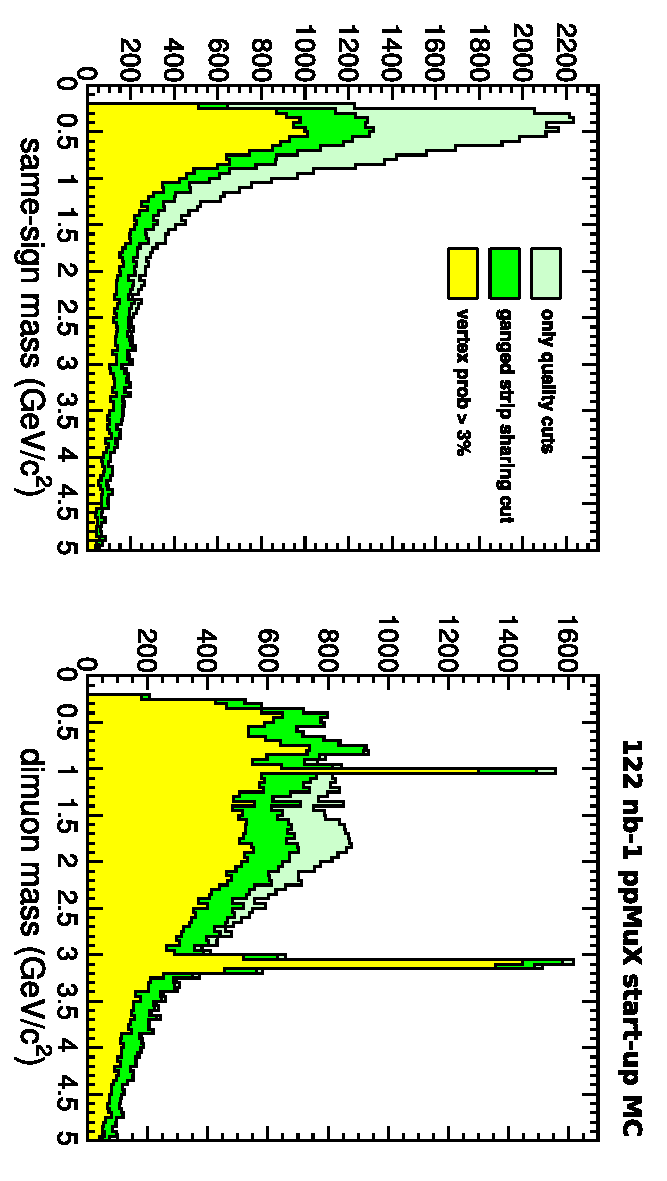
\includegraphics[height=\linewidth, angle=90]{gangedstripcut_mass_MC.pdf}
\end{columns}
\end{frame}

\begin{frame}
\frametitle{Excess in $\phi(1020) \to \mu\mu$}

\begin{itemize}
\item More detail on the $\phi(1020)$ region shows that the excess is
  significant (3.7 sigma)
\begin{itemize}
\item also hint in \href{https://hypernews.cern.ch/HyperNews/CMS/get/muon-performance/531.html}{\scriptsize https://hypernews.cern.ch/HyperNews/CMS/get/muon-performance/531.html}
\end{itemize}

\item Even though $\mathcal{B}(\phi(1020) \to \mu\mu)$ is $2.8\times
  10^{-4}$, observation with 1~nb$^{-1}$ is plausible {\scriptsize (scaling from
  $\phi(1020) \to K^+K^-$, \href{http://cms.cern.ch/iCMS/jsp/db_notes/noteInfo.jsp?cmsnoteid=CMS IN-2010/001}{CMS IN-2010/001})}.
\item Data/MC differences are related to a generator-level $p_T > 2.5$~GeV/$c$ cut on one of the muons in ppMuX (see next slide)
\end{itemize}

\begin{columns}
\column{0.65\linewidth}
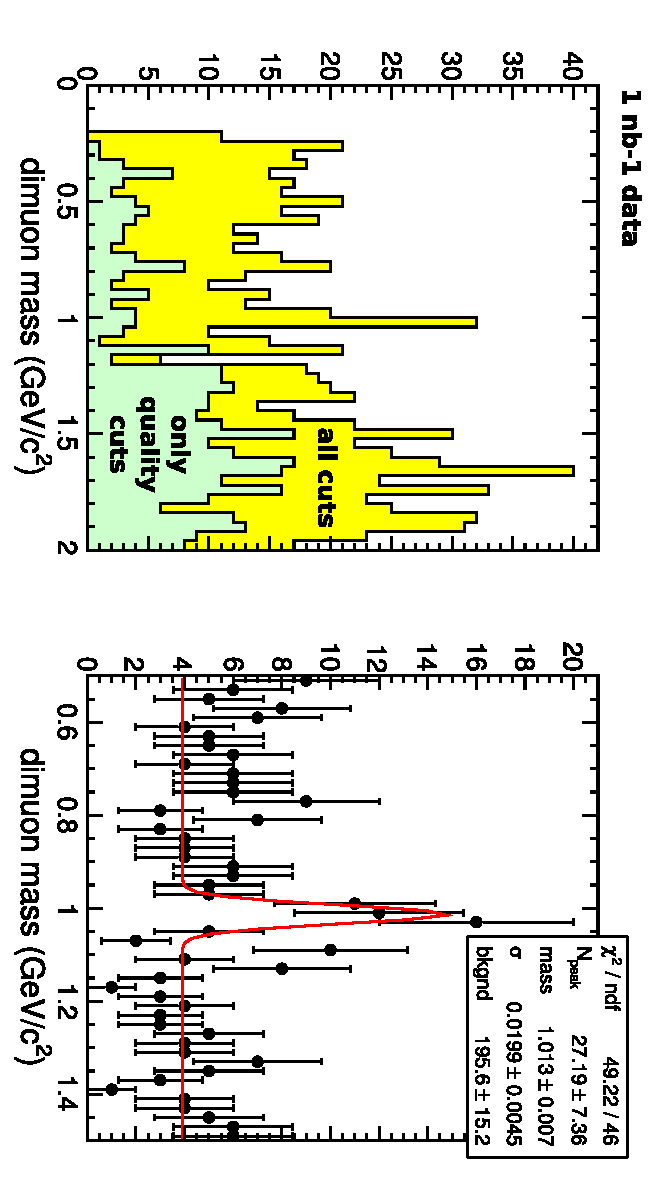
\includegraphics[height=\linewidth, angle=90]{phi_to_mumu.pdf}

\column{0.5\linewidth}
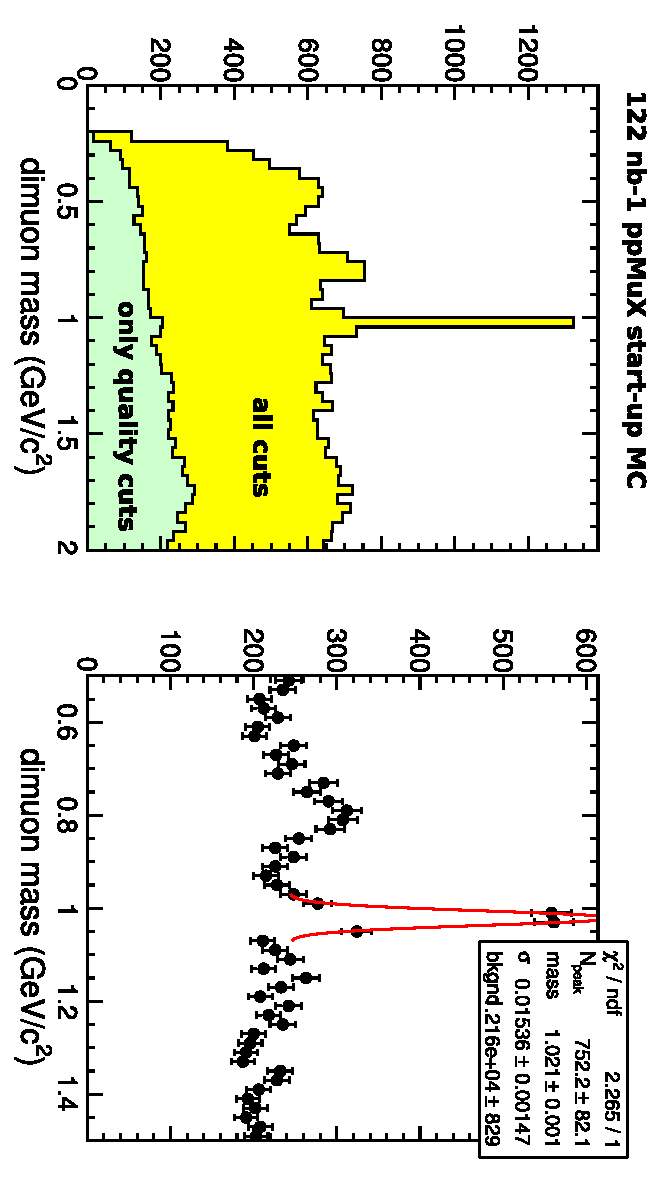
\includegraphics[height=\linewidth, angle=90]{phi_to_mumu_MC.pdf}
\end{columns}
\end{frame}

\begin{frame}
\frametitle{Apples-to-apples comparison}

\begin{itemize}
\item Data/MC differences are related to a generator-level $p_T > 2.5$~GeV/$c$ cut on one of the muons in ppMuX

\item Applying the same cut in data, we lose the $\phi(1020)$ peak but get better agreement between data and MC
\begin{itemize}
\item background levels before and after cuts scale by a factor of 120
\item scaling of signal cannot be tested
\end{itemize}
\end{itemize}

\begin{columns}
\column{0.65\linewidth}
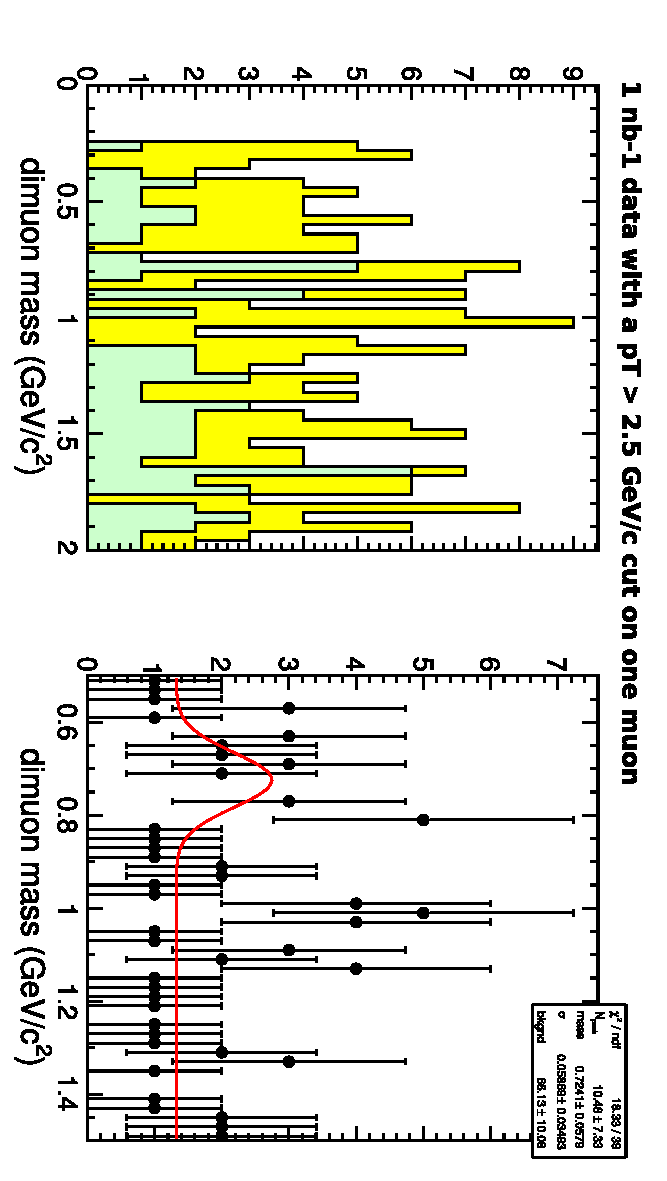
\includegraphics[height=\linewidth, angle=90]{phi_to_mumu_cut25.pdf}

\column{0.5\linewidth}
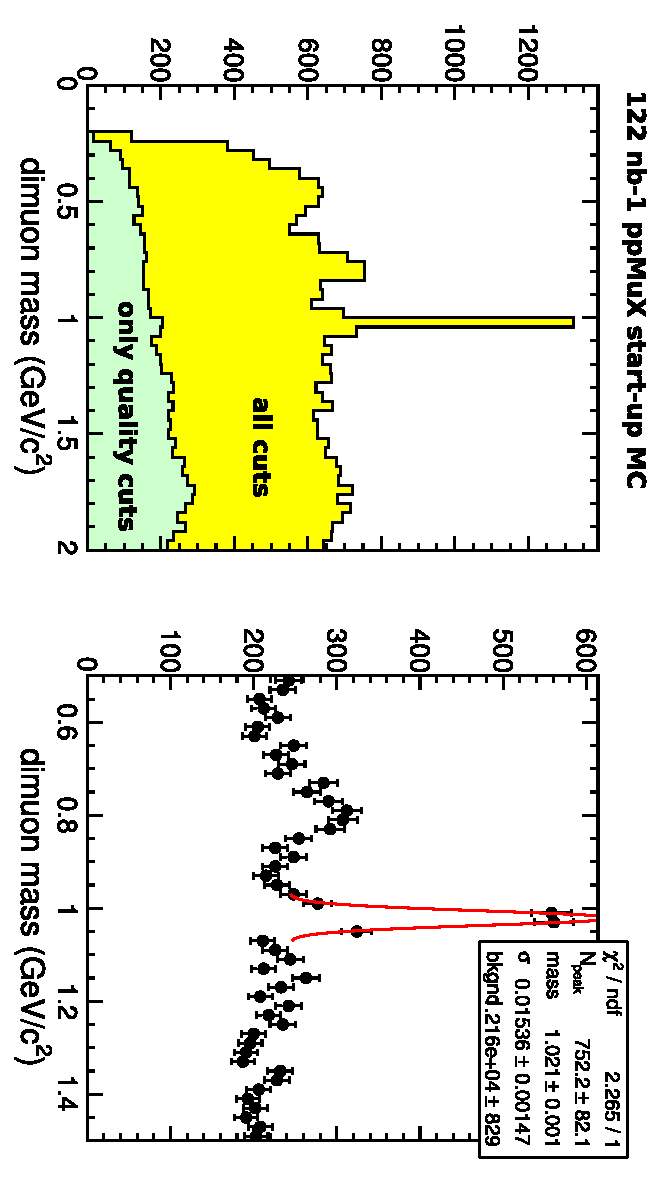
\includegraphics[height=\linewidth, angle=90]{phi_to_mumu_MC.pdf}
\end{columns}
\end{frame}


%% \begin{frame}
%% \frametitle{Outline}
%% \begin{itemize}\setlength{\itemsep}{0.75 cm}
%% \item 
%% \end{itemize}
%% %% \hspace{-0.83 cm} \textcolor{darkblue}{\Large Outline2}
%% \end{frame}

%% \section*{First section}
%% \begin{frame}
%% \begin{center}
%% \Huge \textcolor{blue}{First section}
%% \end{center}
%% \end{frame}

\begin{frame}
\frametitle{Conclusions}

\begin{itemize}\setlength{\itemsep}{0.5 cm}
\item Some physics signatures need to be able to reconstruct close-by muons

\item Primary source of fake close-by muons is a very precise effect from ME1/1a electronics
\begin{itemize}
\item can be cut with high efficiency for real dimuons
\end{itemize}

\item $\phi(1020) \to \mu\mu$ peak is at the level of 3.7~sigma
\end{itemize}

\label{numpages}
\end{frame}

\begin{frame}
\frametitle{One more apples-to-apples}

\begin{itemize}
\item Applying the $p_T > 2.5$~GeV/$c$ cut to same-sign muon pairs for a proper comparison with MC

\item Similar background levels (scaling by 120), but $J/\psi$ appears to be under-produced in MC by a factor of 2.4
\end{itemize}

\begin{columns}
\column{0.65\linewidth}
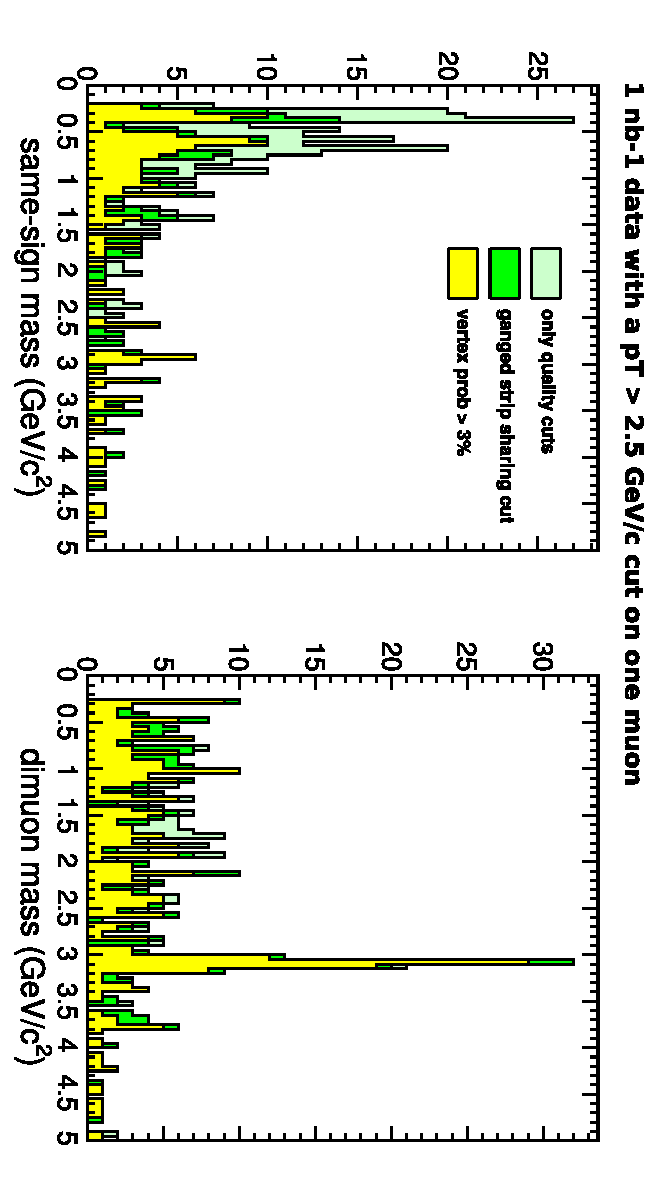
\includegraphics[height=\linewidth, angle=90]{gangedstripcut_mass_cut25.pdf}

\column{0.5\linewidth}
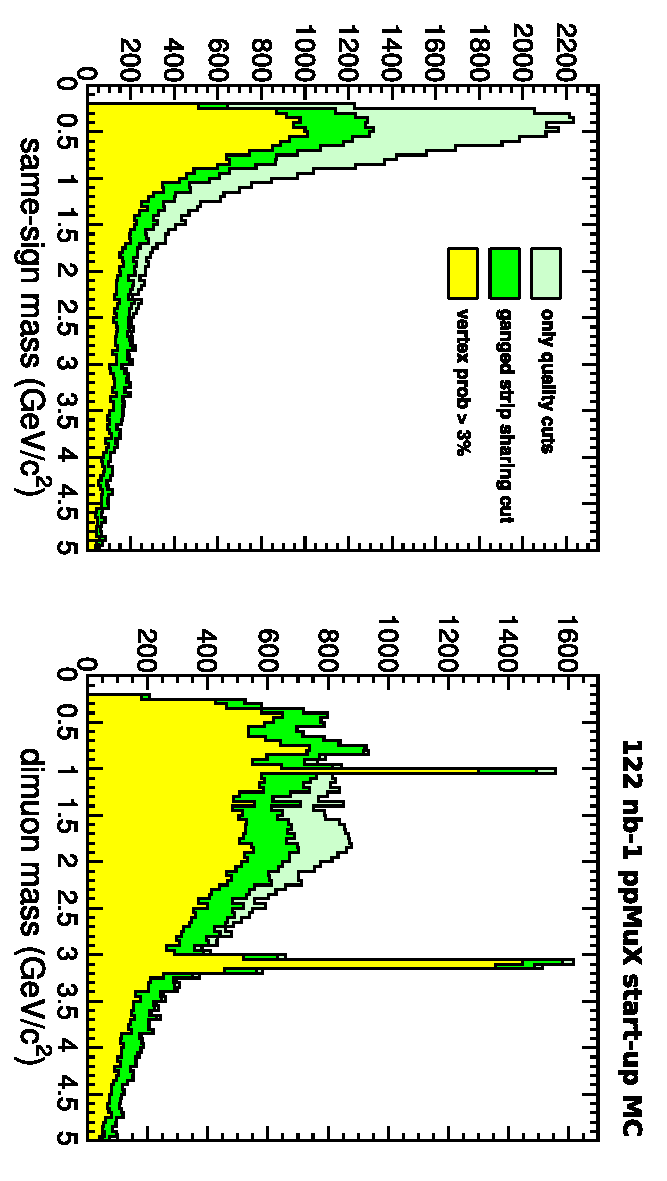
\includegraphics[height=\linewidth, angle=90]{gangedstripcut_mass_MC.pdf}
\end{columns}
\end{frame}

\begin{frame}
\frametitle{Vertex probability cut}

\begin{itemize}
\item Vertex compatibility of the two muons, cut at prob $>$ 3\%
\item This is data
\end{itemize}

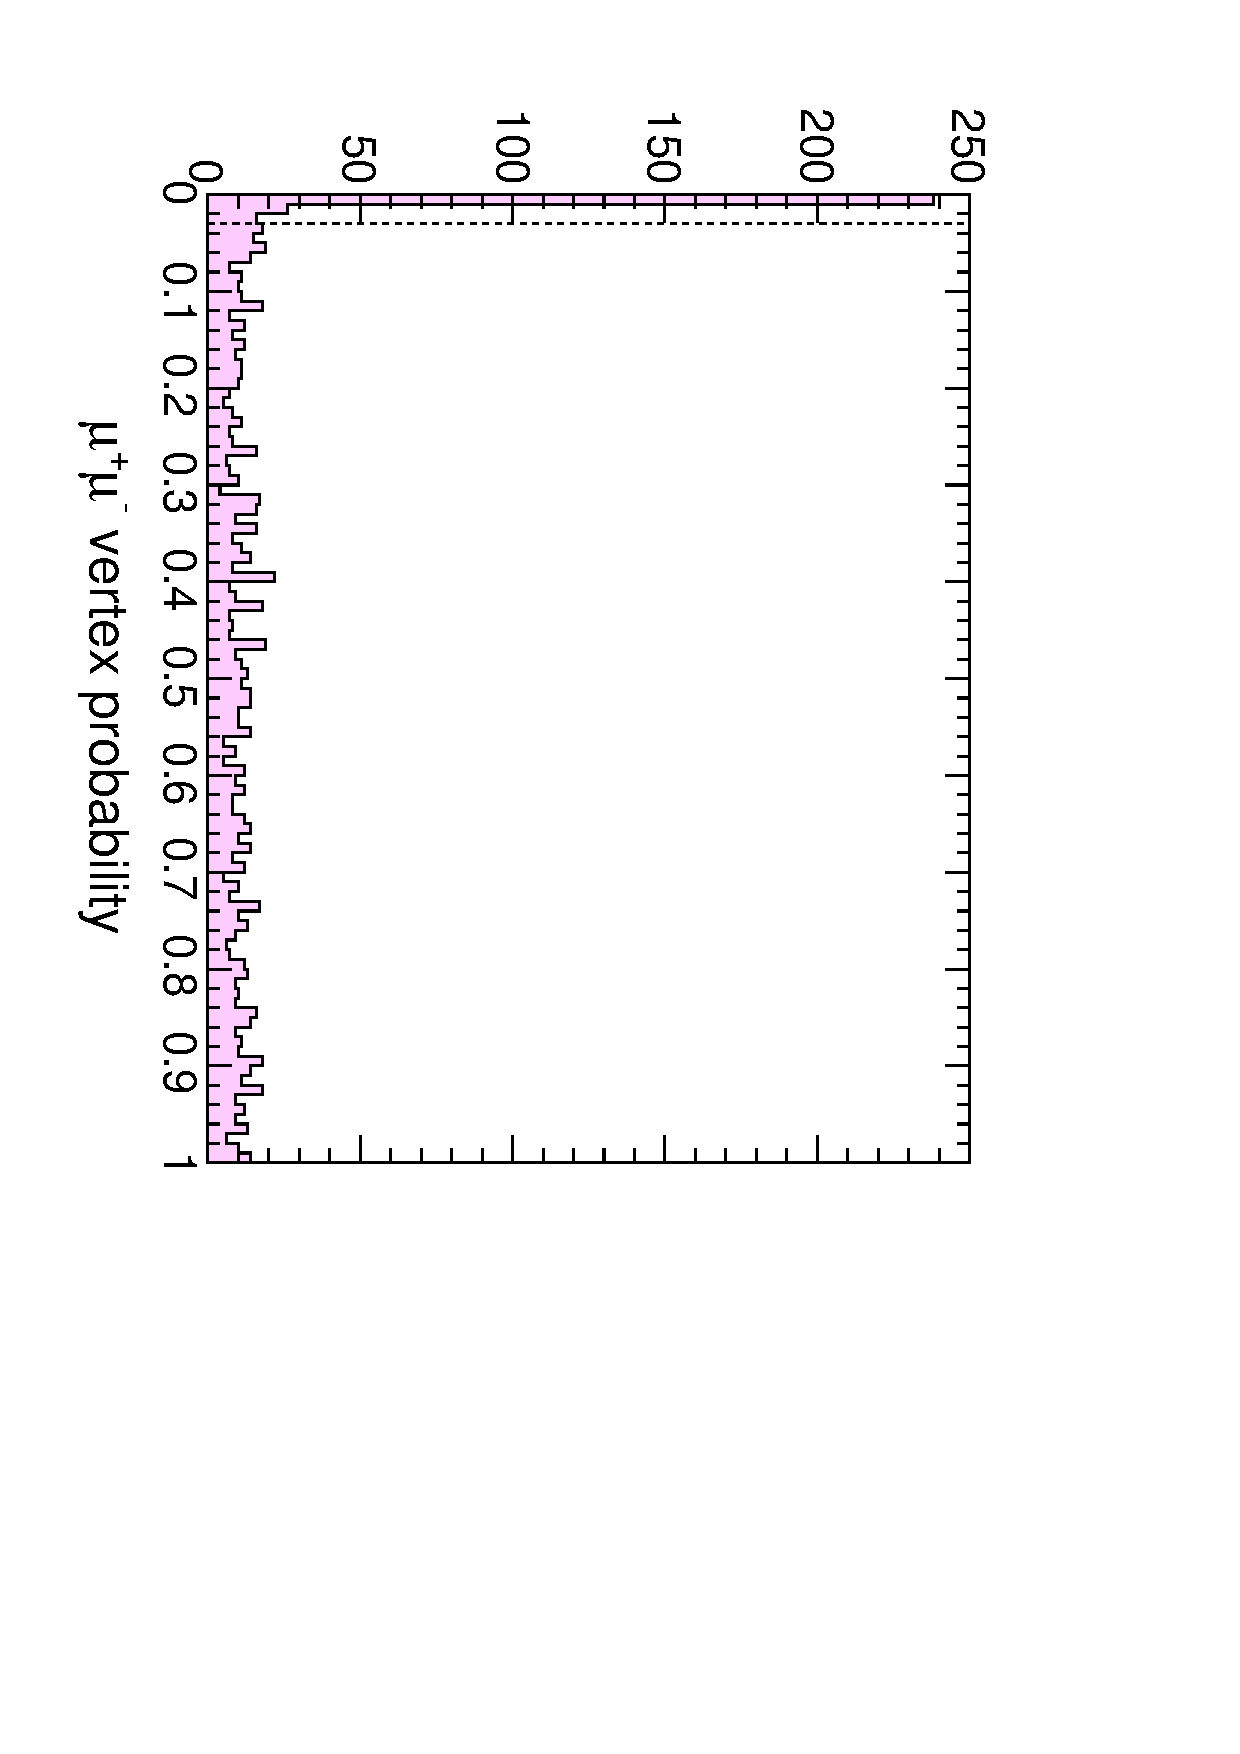
\includegraphics[height=0.5\linewidth, angle=90]{vertexprob.pdf}
\end{frame}

\end{document}
